% !TeX encoding = UTF-8
% !TeX spellcheck = en_US
\section{Getting started}
\IEEEPARstart{T}his project is provided as a set of Eclipse plug-ins.
Depending on if you would like to use the project or just want to explore 
the source code there are different requirements. 
Both development and runtime execution have been tested under {\it Eclipse Modeling Luna SR2} 
and {\it Eclipse Modeling Mars.2 Release (4.5.2)} on AMD64 architecture with a Linux operating system 
and at least 8 GB RAM. 
\\ \ \\
\warning{}
This is a prototype / proof-of-concept and is not intended to be used in production environments!!!
It may contain some serious bugs, security issues or design flaws which might lead to data loss or data corruption. 
You have been warned ;-). 

\subsection{How-To use}\label{sec:howToUse}
\begin{enumerate}
 \item Ensure that you have Git installed and that the git executable is in your current \$PATH variable.
 \item\label{howToUseDownload} Download Eclipse Modeling IDE from 
 \begin{itemize}
  \item either \url{https://eclipse.org/downloads/}\cite{Eclipse_1}
  \item or \url{https://eclipse.org/downloads/packages/release/luna/sr2}\cite{Eclipse_2}
 \end{itemize}
 \item Unzip and open the Eclipse IDE
 \item Install Eclipse Modisco (Help$\rightarrow$Install new software, 
 select the predefined software site {\it Modeling package updates for Eclipse Mars}\cite{Eclipse_3}
 or {\it Modeling package updates for Eclipse Luna}\cite{Eclipse_4}
 and install either {\it Modisco/Modisco SDK (incubation) 0.13.2.201601200708}
 or {\it Modeling/Modisco SDK (Incubation) 0.12.2.201501021045} (depending on your Eclipse version). 
 \item Install NeoEMF by opening the install new software dialog again and add 
  \url{https://timeraider4u.github.io/NeoEMF/}\cite{Eclipse_5} as NeoEMF update site. Install
  \begin{itemize}
   \item {\it Base/NeoEMF Persistence framework}
   \item {\it Backends/NeoEMF Blueprints adapter}
   \item and {\it Backends/NeoEMF Blueprints implementation}
  \end{itemize}
  each with version 0.0.1.2016040202
  \item Install {\it org.xtext.antlr.generator} 
  by adding \url{https://timeraider4u.github.io/org.xtext.antlr.generator/}\cite{Eclipse_6} 
  as an update site and selecting the feature {\it org.xtext.antlr.generator/org.xtext.antlr.generator.feature} 
  with version 3.2.1.201604141818.
  \item\label{howToUseXtextInstall} Install the modified version of {\it Xtext}
  by adding \url{https://timeraider4u.github.io/xtext/}\cite{Eclipse_7} as an update site 
  and select {\it Xtext/Xtext Complete SDK 2.9.0.v201604150031}
  \item\label{howToUseKefaxInstall} Install KeFax by adding \url{https://timeraider4u.github.io/kefax/}\cite{Kefax_URL}
  as an update site and select {\it at.jku.weiner.kefax/at.jku.weiner.kefax} with version 0.1.0.201605080110
  \item Your installed software (Help$\rightarrow$About Eclipse$\rightarrow$Installation Details) 
  should now look similiar to the screenshot shown in figure \ref{fig:EclipseInstall}:
  \begin{figure*}[ht]
    \centering
	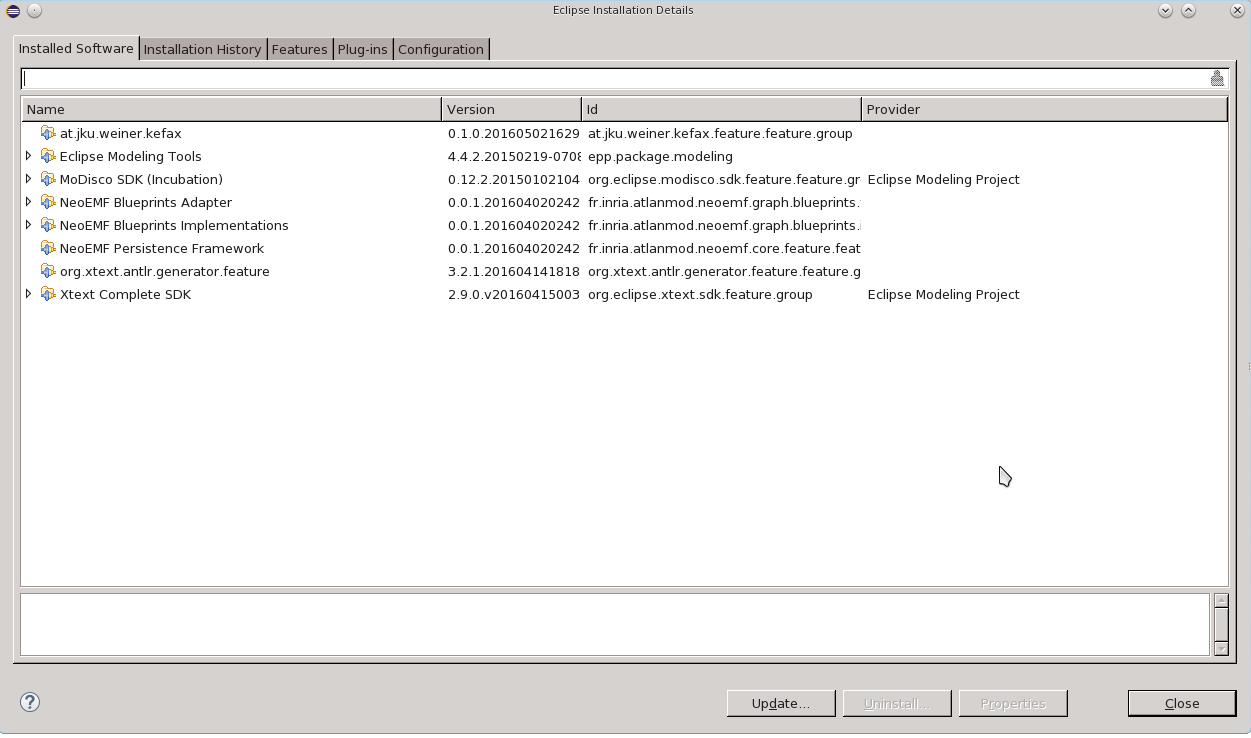
\includegraphics[scale=0.5]{images/install-software}
	\caption{Installation details}
    \label{fig:EclipseInstall}
  \end{figure*}
  \FloatBarrier
  \item Edit the eclipse.ini file. It should contain the following configuration:
  \lstinputlisting[frame=single,extendedchars=true,label=eclipseINI,caption={part of the eclipse.ini},
  breaklines=true,]{code/eclipse.ini}
  \item\label{howToUseRestart} Restart Eclipse
  \item Run by selecting menu items from {\it KeFaX} menu (shown in figure \ref{fig:KefaxMenu}) either
    \begin{itemize}
     \item KeFax $\rightarrow$Run KeFax demonstration A
     \item or KeFax $\rightarrow$Run KeFax demonstration B
    \end{itemize}
\end{enumerate}

 \begin{figure}[ht]
  \centering
  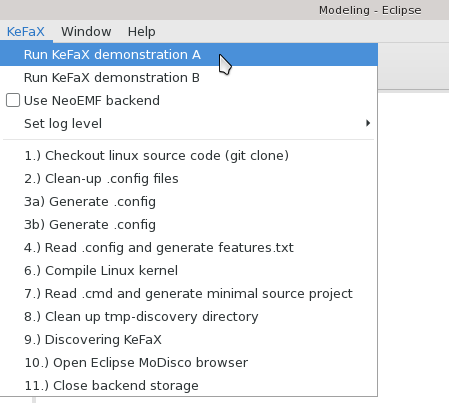
\includegraphics[scale=0.5]{images/kefax-menu-0002}
  \caption{Using KeFaX after installation}
  \label{fig:KefaxMenu}
  \end{figure}
This will now download the Linux source code with git, 
generating a minimal working configuration file, 
execute a kernel compilation to obtain the compile 
options for all source files, generate a {\it features.txt}
file in the destination project {\it kefax-linux-working}, 
copy the minimal required source and header files to the 
{\it kefax-linux-working project} and start discovering the {\it kefax-linux-working project}.
Once pre-processing and parsing is done, 
KeFax will open the {\it MoDisco EMF browser} which shows the 
reverse-engineered Linux kernel C source model. 

Demonstration mode A and demonstration mode B just differ by one feature: 
B has {\it CONFIG\_UNIX98\_PTYS} set to yes will while is not set for A at all. 
This is either done in step {\it 3a) Generate .config} or in step {\it 3b) Generate .config} of the {\it KeFaX} menu. 

The resulting EMF model file(s) can than be found in the folder {\it tmp-discover} of the {\it kefax-linux-working} project. 
\\ \ \\
\begin{figure*}[ht]
  \centering
  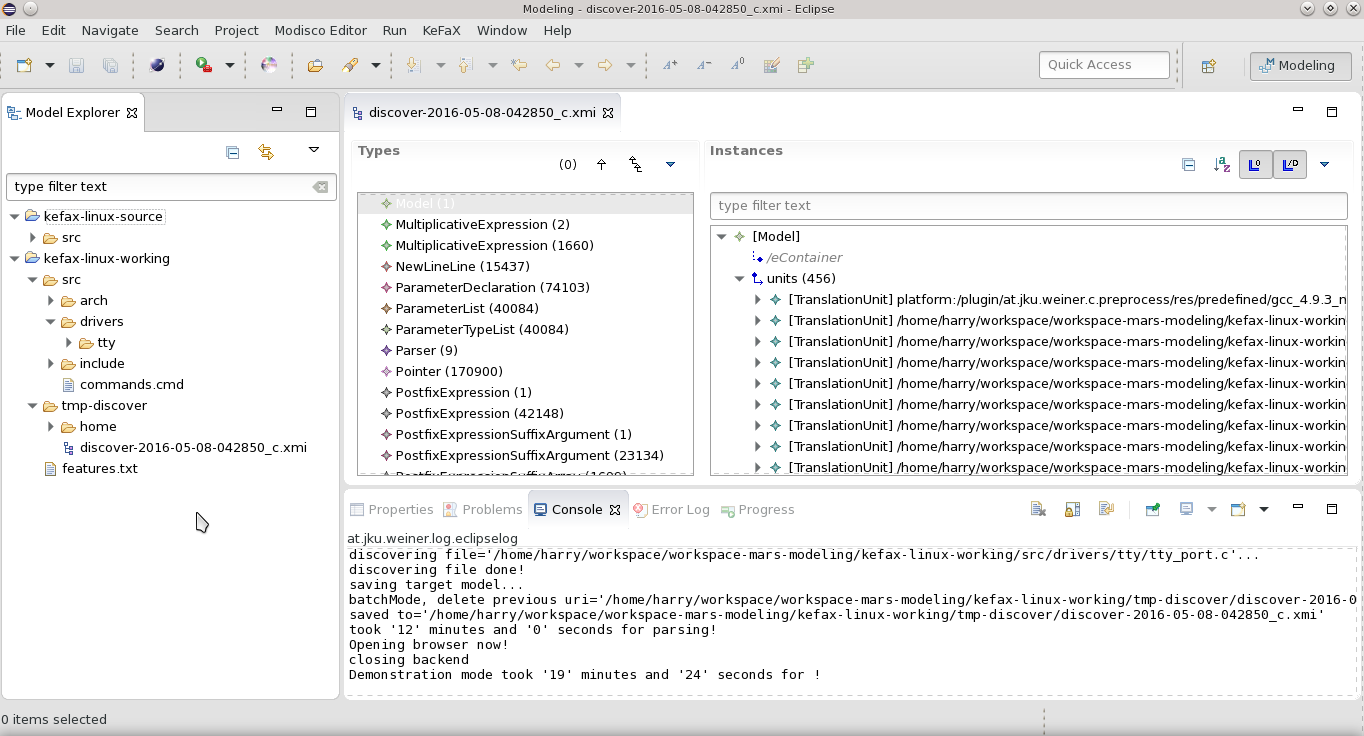
\includegraphics[scale=0.5]{images/discoverer-2015-05-08}
  \caption{Result after running KeFaX}
  \label{fig:discoverer20150508}
\end{figure*}

You might also adjust the log-level or run the individual commands step-wise to see what they are doing in detail.
\\ \ \\
\warning{} Do not run with log-level set to {\it trace}. 
Log-level {\it trace} is only meant to be used for debugging very nasty bugs 
(e.g., preprocessor macro expansion).
It will take almost forever to execute the preprocessor due to printing the detailed log to the console.
Use at your own risk\dots{} You have been warned ;-).

\FloatBarrier

\subsection{How-To develop}
The whole project is distributed under Eclipse Public License - v 1.0 
\cite{EPL_URL} unless otherwise stated.
The source code can be obtained  with git from \url{https://github.com/timeraider4u/kefax}\cite{Kefax2_URL}
\begin{enumerate}
 \item \begin{lstlisting}[language=Bash,breaklines=true,]
        git clone https://github.com/timeraider4u/kefax
       \end{lstlisting}
 \item Execute steps \ref{howToUseDownload} -- \ref{howToUseXtextInstall} from How-To use \ref{sec:howToUse}
 \item Add \url{https://timeraider4u.github.io/kefax/}\cite{Kefax_URL} as an update site, 
 just like in step \ref{howToUseKefaxInstall} of How-To use, but instead of installing {\it kefax} 
 select {\it at.jku.weiner.xtexttest/at.jku.weiner.xtexttest version 0.1.0.201605080110}
 \item Restart Eclipse
 \item Import project into workspace (File $\rightarrow$ Import $\rightarrow$ General $\rightarrow$ 
 Existing projects into workspace) and select the workspace folder inside the local {\it kefax}
 git repository as the root directory. Select all projects and start the import process.
 \item 6. If there are any errors/failures shown after importing you may try to execute 
 Project $\rightarrow$ Clean $\rightarrow$ Clean all projects.
 This will remove temporary Xtext/Xtend files and enforce a global rebuild.
 \item The code structuring will be explained later in this paper. 
 \item KeFaX uses Maven (and Github Travis) for continuous integration:
 A local Maven 3.0 build can be started by navigating to the local kefax git repository root and executing 
 \item \begin{lstlisting}[language=Bash,breaklines=true,]
 mvn clean install
 \end{lstlisting}. This will also execute all JUnit tests.
 \item Feel free to start a pull request or report an issue on the Github page \cite{Kefax2_URL}.
  \begin{itemize}
   \item The {\it master} branch is used for development
   \item The {\it gh-pages} branch is used to store the Eclipse update site. 
  \end{itemize}
 \item Also take a look at the {\it README.md} file 
 and execute git pull from time to time to keep in touch with the latest changes. 
\end{enumerate}
